\documentclass{resume}
%Russian-specific packages
%--------------------------------------
%--------------------------------------

\begin{document}

\fontfamily{ppl}\selectfont

\noindent
\begin{tabularx}{\linewidth}{@{}m{0.8\textwidth} m{0.2\textwidth}@{}}
{
    \Large{Орлов Александр} \newline
    \small{
        \clink{
            \href{mailto:ayuorlov_1@edu.hse.ru}{ayuorlov\_1@edu.hse.ru} \textbf{·}
            {\fontdimen2\font=0.75ex +79299313162}
        } \newline
        Королёв, Московская область
    }
} &
{
    \hfill
    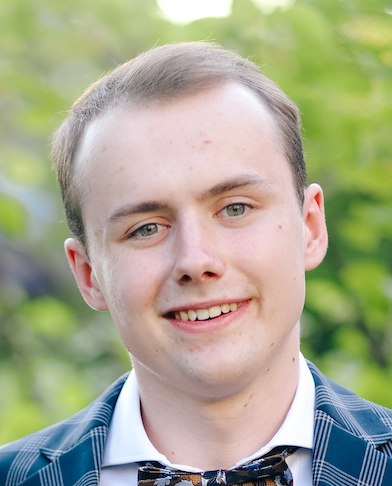
\includegraphics[width=3cm]{images/111.png}
}
\end{tabularx}
\begin{center}
\begin{tabularx}{\linewidth}{@{}*{2}{X}@{}}
% left side %
{
    \csection{Образование}{\small
        \begin{itemize}
            % item 1 %
            \item \frcontent{Прикладная математика и информатика, GPA: 8.43/10}{Высшая Школа Экономики, ФКН}{}{2023}
            \item \frcontent{Лицей научно-инжереного профиля}{Королёв}{}{2019}
        \end{itemize}
    }
    \csection{Опыт и Достижения}{\small
        \begin{itemize}
            % item 3 %
            \item \frcontent{Летняя школа по биоинформатике}{Участник}{}{2020, 2021}
            \item \frcontent{Введение в молекулярную биологию}{Stepik}{}{2019}
            % item 1 %
            \item \frcontent{Победитель и призер олимпиад школьников по математике}{Ломоносов, Курчатов, Физтех, РЭ ВОШ}{}{2019}
            % item 2 %
            \item \frcontent{Призер олимпиад школьников по физике}{Росатом, Ломоносов}{}{2019}

        \end{itemize}
    }
}
% end left side %
&
% right side %
{
    \csection{Навыки}{\small
        \begin{itemize}
            \item \textbf{Технологии} \newline
            {\footnotesize Python, NumPy, Scipy, SQL, Linux, Bash, Git, LaTeX, MEGA, PyMol, C++, gdb}{}{}
            \item \textbf{Математические предметы} \newline
            {\footnotesize Линейная алгебра и геометрия, Теория вероятностей, Матричные вычисления, Математический анализ, Дискретная математика, Дифференциальные уравнения,  Математическая статистика (в процессе прохождения университетского курса) }{}{}
        \end{itemize}
    }
    \csection{Проекты}{\small
        \begin{itemize}
            \item \frcontent{IQ-Beat}{Стажер в проекте по анализу ЭКГ сигналов}{}{Python, Bash, NumPy, Scipy, Pandas, Git}
            \item \frcontent{Веб-приложение агрегатор преподавателей}{Python, Django, sqlite3}{}{}
        \end{itemize}
    }
    \csection{Интересы}{\small
        \begin{itemize}
            \item {\footnotesize Решение интересных задач}
            \item {\footnotesize Математика}
            \item {\footnotesize Биология}
            \item {\footnotesize Путешествия}
        \end{itemize}
    }
}

\end{tabularx}
\end{center}
\csection{О себе}{\small
\begin{spacing}{1}
\noindent
\begin{itemize}
            \item {\footnotesize Студент 2 курса ПМИ ФКН ВШЭ. Увлекаюсь математикой, анализом данных и их приложениями к биологии}
            \item {\footnotesize В свободное от учебы время занимаюсь
изучением биоинформатики, молекулярной биологии, анализом ЭКГ в рамках проекта или отдыхаю за просмотром кино}
            \item {\footnotesize Любимые математические предметы: теория вероятностей, матричные вычисления, дискретная математика; Любимые биологические предметы: молекулярная биология, микробиология}
            \item {\footnotesize Прошел факультатив по функциональному анализу, сейчас прохожу факультатив по дополнительным главам теории вероятностей. Прохожу майнор по биоинформатике. После майнора научился пользоваться программами BLAST, MEGA, PyMol, знаю основные алгоритмы выравнивания последовательностей (программировал некоторые из них на Летней школе по биоинформатике), знаю основные идеи алгоритмов, лежащих в основе предсказания генов. Еще со школы очень люблю биологию и хочу учиться использовать свои знания в этой области!}
\end{itemize}
\end{spacing}
}


\end{document}